\chapter{Daur Biogeokimia}\label{ch:b2:biogeochemical-cycles}

Pada bulan Maret 1958 seorang ahli kimia muda bernama Charles Keeling
menyalakan sebuah penganalisis gas inframerah di lereng utara Mauna
Loa, di Hawaii, tiga setengah kilometer di atas Pasifik, tempat
udaranya tercampur sebaik yang dapat dicapai udara. Ia telah
mengharapkan mengukur sebuah tetapan; dalam setahun ia memiliki sebuah
gigi gergaji --- karbon dioksida yang naik tiap musim dingin dan turun
tiap musim panas ketika hutan belahan bumi utara mengembuskan dan
menarik napas --- dan dalam beberapa tahun sebuah kemiringan di bawah
gigi gergajinya yang tidak berhenti sejak itu. \omterm{prop:b2:biogeochemical-cycles:carbon}{Kurva Keeling} adalah
pernapasan biosfer yang terlihat dari luar, dengan sebuah bagan demam
tergambar di atasnya. Bab ini membahas daur yang dicatat kurvanya: di
mana karbon, nitrogen, fosfor, dan belerang makhluk hidup tersimpan,
seberapa cepat semuanya berpindah antartandon, apa yang menetapkan
kecepatan itu --- yang sebagian besarnya adalah metabolisme pada
\cref{ch:b2:microbial-metabolism} --- dan apa yang telah dikerjakan
satu spesies terhadap tiap daurnya dalam dua ratus tahun.

\section{Tandon, fluks, dan waktu tinggal}

\begin{definition}[Tandon, fluks, waktu tinggal]\label{def:b2:biogeochemical-cycles:reservoir}
\index{tandon}\index{fluks}\index{waktu tinggal}\index{keadaan tunak}\index{daur biogeokimia}
Sebuah \emph{daur biogeokimia} adalah perpindahan sebuah unsur
antar\emph{tandon} (atmosfernya, lautannya, tanahnya, biomassa
hidupnya, batuannya) lewat \emph{fluks} yang diukur dalam massa tiap
tahun. Sebuah tandon bermassa $M$ dengan aliran keluar total $F$
memiliki \emph{waktu tinggal} $\tau = M/F$, yaitu waktu rerata sebuah
atom berada di dalamnya; pada \emph{keadaan tunak} aliran masuknya sama
dengan aliran keluarnya dan $M$ tetap. Daurnya tergandeng lewat
stoikiometri kehidupan --- \emph{nisbah Redfield} plankton laut,
$\mathrm{C:N:P} =
106:16:1$ menurut atomnya --- sehingga pasokan unsur
yang paling langka menetapkan laju penyerapan semua unsur lainnya.
\end{definition}

\begin{theorem}[Model satu kotak]\label{thm:b2:biogeochemical-cycles:box}
\index{model kotak}\index{waktu kendur}
Jika sebuah \omterm{def:b2:biogeochemical-cycles:reservoir}{tandon} kehilangan isinya pada laju yang sebanding dengan
apa yang ia tahan, $F_{\text{keluar}} = M/\tau$, dan menerima sebuah
aliran masuk yang tetap $F_{\text{masuk}}$, maka
\[
\frac{\mathrm{d}M}{\mathrm{d}t} = F_{\text{masuk}} - \frac{M}{\tau},
\qquad
M(t) = M^{*} + (M_0 - M^{*})\,e^{-t/\tau}, \qquad M^{*} = F_{\text{masuk}}\tau :
\]
\omterm{def:b2:biogeochemical-cycles:reservoir}{tandonnya} mengendur menuju sebuah \omterm{def:b2:biogeochemical-cycles:reservoir}{keadaan tunak} yang sebanding dengan
masukannya, dengan \omterm{def:b2:biogeochemical-cycles:reservoir}{waktu tinggalnya} sebagai tetapan waktunya. Sebuah
kenaikan bertangga pada masukannya menaikkan \omterm{def:b2:biogeochemical-cycles:reservoir}{keadaan tunaknya} secara
sebanding dan \omterm{def:b2:biogeochemical-cycles:reservoir}{tandonnya} mengikutinya dalam beberapa $\tau$: sebuah
lungkang dengan \omterm{def:b2:biogeochemical-cycles:reservoir}{waktu tinggal} beberapa hari (amonia atmosfer, nitrat
sebuah danau pada musim semi) mengikuti sumbernya; sedangkan yang
\omterm{def:b2:biogeochemical-cycles:reservoir}{waktu tinggalnya} berabad-abad (karbon laut dalam, bahan organik
tanahnya) memadukannya, dan usikan sebuah lungkang yang lambat berumur
lebih panjang daripada usikan yang menyebabkannya.
\end{theorem}
\begin{proof}
Persamaannya lurus dengan koefisien yang tetap: \omterm{def:b2:biogeochemical-cycles:reservoir}{keadaan tunaknya}
$M^{*}$ membuat ruas kanannya nol, dan simpangannya $m = M - M^{*}$
mematuhi $\dot m = -m/\tau$, sehingga $m = m_0 e^{-t/\tau}$. Jika
sebuah \omterm{def:b2:biogeochemical-cycles:reservoir}{tandon} memiliki beberapa aliran keluar, $\tau$ ditetapkan
jumlahnya, $1/\tau = \sum_i
1/\tau_i$: lubuk yang tercepat menguasai.
\end{proof}

\section{Daur karbonnya}

\begin{proposition}[Anggaran karbonnya]\label{prop:b2:biogeochemical-cycles:carbon}
\index{daur karbon}\index{bagian yang mengudara}\index{lubuk karbon}\index{kurva Keeling}
Dalam satuan gigaton karbon (\unit{GtC}, $10^{12}$~kg), \omterm{def:b2:biogeochemical-cycles:reservoir}{tandon}
utamanya adalah atmosfernya (kira-kira 880 pada tahun 2020-an, 590
sebelum industrinya), tumbuhan daratnya (450), tanahnya (1700), laut
permukaannya (900), laut dalamnya (\num{37000}), dan batuan endapannya
(\num{e8}); bahan bakar fosilnya adalah bagian dari yang terakhir yang
dapat dijangkau industrinya, yaitu sekitar \num{5000}. \omterm{def:b2:biogeochemical-cycles:reservoir}{Fluks} alaminya
besar dan hampir berimbang: fotosintesis di daratan mengambil kira-kira
120 tiap tahun dan respirasi serta penguraiannya mengembalikannya;
permukaan lautnya bertukar kira-kira 80 tiap arahnya dengan udaranya.
\omterm{def:b2:biogeochemical-cycles:reservoir}{Fluks} manusianya kecil terhadap semuanya ini --- sekitar 10 tiap tahun
dari bahan bakar fosil dan 1 dari penggundulan hutan --- tetapi searah,
dan atmosfernya telah menahan \emph{kira-kira \qty{45}{\%}} darinya
(yaitu \emph{\omterm{prop:b2:biogeochemical-cycles:carbon}{bagian yang mengudara}}), dengan lautnya mengambil
seperempat dan daratannya, yang dipupuk $\mathrm{CO_2}$ tambahannya,
mengambil sisanya. Satu bagian tiap sejuta $\mathrm{CO_2}$ atmosfer adalah
\qty{2.13}{GtC}; kepekatannya naik dari 280 menjadi \num{315}~ppm
antara tahun 1750 dan 1958, dan dari 315 menjadi di atas \num{420}
antara tahun 1958 dan tahun 2020-an, kini sebesar \qty{2.5}{ppm} tiap
tahun. \omterm{def:b2:biogeochemical-cycles:reservoir}{Waktu tinggal} sebuah molekul $\mathrm{CO_2}$ di udaranya, $880/200 \approx 4$ tahun, itu pendek; umur \emph{kelebihannya}, yang ditetapkan
pencampuran lambat ke dalam laut dalamnya dan pelapukan batuannya yang
lebih lambat lagi, berabad-abad sampai beribu tahun --- seperlima dari
yang dipancarkan hari ini masih akan berada di udaranya dalam sepuluh
ribu tahun.
\end{proposition}
\begin{proof}[Bukti eksperimental]
Tiga tanda tangan memperlihatkan bahwa karbon yang ditambahkan itu
fosil. Isotopnya: karbon fosil tidak memiliki $\mathrm{{}^{14}C}$ (ia
telah meluruh jutaan tahun yang lalu) dan miskin $\mathrm{{}^{13}C}$
seperti seluruh karbon tumbuhan, dan atmosfernya telah kehilangan
keduanya --- yaitu efek Suess, yang terukur pada lingkaran pohon sejak
tahun 1950-an. Oksigennya: $\mathrm{O_2}$ atmosfernya turun seiring,
menurut stoikiometri pembakarannya, sebagaimana ditunjukkan putra
Keeling pada tahun 1990-an, yang tidak akan dihasilkan sebuah sumber
gunung api atau sumber laut. Pembukuannya: jumlah batu bara, minyak,
dan gas yang terjual, yang diubah menjadi karbon, melampaui kenaikan di
udaranya dengan faktor dua, dan separuh yang hilangnya ditemukan pada
karbon anorganik terlarut lautnya yang naik dan pH-nya yang turun,
serta pada lubuk daratannya. Gigi gergaji musimannya, yang lebih besar
di Barrow di Alaska daripada di Mauna Loa dan nyaris tidak ada di Kutub
Selatan, adalah penyerapan musim panas dan pelepasan musim dingin hutan
utaranya --- sebuah pengukuran langsung pernapasan biosfernya.
\end{proof}

\begin{omfigure}
\begin{tikzpicture}
\begin{axis}[
  width=0.9\linewidth, height=6cm,
  axis x line=bottom, axis y line=left,
  xmin=1955, xmax=2026, ymin=300, ymax=430,
  xlabel={tahun}, ylabel={$\mathrm{CO_2}$ (ppm), rerata tahunan Mauna Loa},
  xlabel style={font=\small, at={(axis description cs:0.5,-0.13)}, anchor=north},
  ylabel style={font=\small},
  tick label style={font=\small}, xtick={1960,1970,1980,1990,2000,2010,2020}, ytick={300,325,350,375,400,425},
  scaled x ticks=false, x tick label style={/pgf/number format/1000 sep=},
  clip=false,
]
\addplot[very thick, omDef, mark=*, mark size=1pt] coordinates {
(1959,316.0) (1962,318.5) (1965,320.0) (1968,323.0) (1971,326.3) (1974,330.2) (1977,333.8) (1980,338.8) (1983,342.8) (1986,347.2) (1989,353.1) (1992,356.4) (1995,360.8) (1998,366.7) (2001,371.1) (2004,377.5) (2007,383.8) (2010,389.9) (2013,396.5) (2016,404.2) (2019,411.4) (2022,418.5) (2024,424.6)};
\node[font=\scriptsize, anchor=north west, align=left] at (axis cs:1958,425) {tahun 1960-an: \qty{+0.9}{ppm/yr}\\tahun 2010-an: \qty{+2.4}{ppm/yr}};
\node[font=\scriptsize, anchor=west, align=left] at (axis cs:1990,320) {aras praindustri: \qty{280}{ppm};\\tiap tahun gigi gergaji $\pm\qty{3}{ppm}$ menumpangi garis ini};
\end{axis}
\end{tikzpicture}

{\small \omterm{prop:b2:biogeochemical-cycles:carbon}{Kurva Keeling}: rerata tahunan karbon dioksida di udara Mauna
Loa sejak tahun 1959. Kemiringannya nyaris melipat tiga; gigi gergaji
musiman di atasnya, yang tidak diperlihatkan pada skala ini, adalah
fotosintesis musim panas belahan bumi utaranya.}
\end{omfigure}

\begin{omfigure}
\begin{tikzpicture}[every node/.style={font=\scriptsize}, >=stealth, box/.style={draw, rounded corners, minimum width=2.2cm, minimum height=0.9cm, align=center, fill=#1}]
  \node[box=omDef!15] (atm) at (0,3) {atmosfer\\880};
  \node[box=omThm!15] (veg) at (-4.4,0.6) {tumbuhan darat 450\\tanah 1700};
  \node[box=omProp!15] (surf) at (4.4,0.6) {laut permukaan\\900};
  \node[box=omProp!25] (deep) at (4.4,-1.6) {laut dalam\\37\,000};
  \node[box=gray!20] (rock) at (0,-1.6) {batuan dan bahan bakar fosil\\$10^{8}$; terjangkau $\sim 5000$};
  \draw[->, thick] ([xshift=-2mm]atm.south west) -- node[above left, pos=0.45] {120 fotosintesis} ([xshift=-4mm]veg.north);
  \draw[->, thick] ([xshift=5mm]veg.north) -- ([xshift=-2mm]atm.south); \node[anchor=north east] at (-0.4,1.5) {119 respirasi, kebakaran};
  \draw[->, thick] ([xshift=2mm]atm.south east) -- node[above right, pos=0.45] {80 pelarutan} ([xshift=4mm]surf.north);
  \draw[->, thick] ([xshift=-5mm]surf.north) -- ([xshift=2mm]atm.south); \node[anchor=north west] at (0.4,1.5) {78 pengeluaran gas};
  \draw[<->, thick] (surf) -- node[right] {$\sim 100$ pencampuran, penenggelaman} (deep);
  \draw[->, very thick, omExo!80!black] (rock.north) -- node[left, align=right, pos=0.4] {10 bahan bakar fosil\\ + 1 tata guna lahan} (atm.south);
  \node[align=left, anchor=west] at (7.0,3.2) {fluks dalam \unit{GtC/yr},\\ stok dalam \unit{GtC}\\[2pt] dari 11 yang dipancarkan:\\ 5 tinggal di udara,\\ 3 masuk ke daratan,\\ 3 masuk ke lautan};
\end{tikzpicture}

{\small \omterm{prop:b2:biogeochemical-cycles:carbon}{Daur karbonnya} dalam angka bulat. Pertukaran alaminya sepuluh
kali \omterm{def:b2:biogeochemical-cycles:reservoir}{fluks} manusianya, tetapi pertukarannya hampir saling meniadakan;
\omterm{def:b2:biogeochemical-cycles:reservoir}{fluks} manusianya tidak.}
\end{omfigure}

\begin{omfigure}
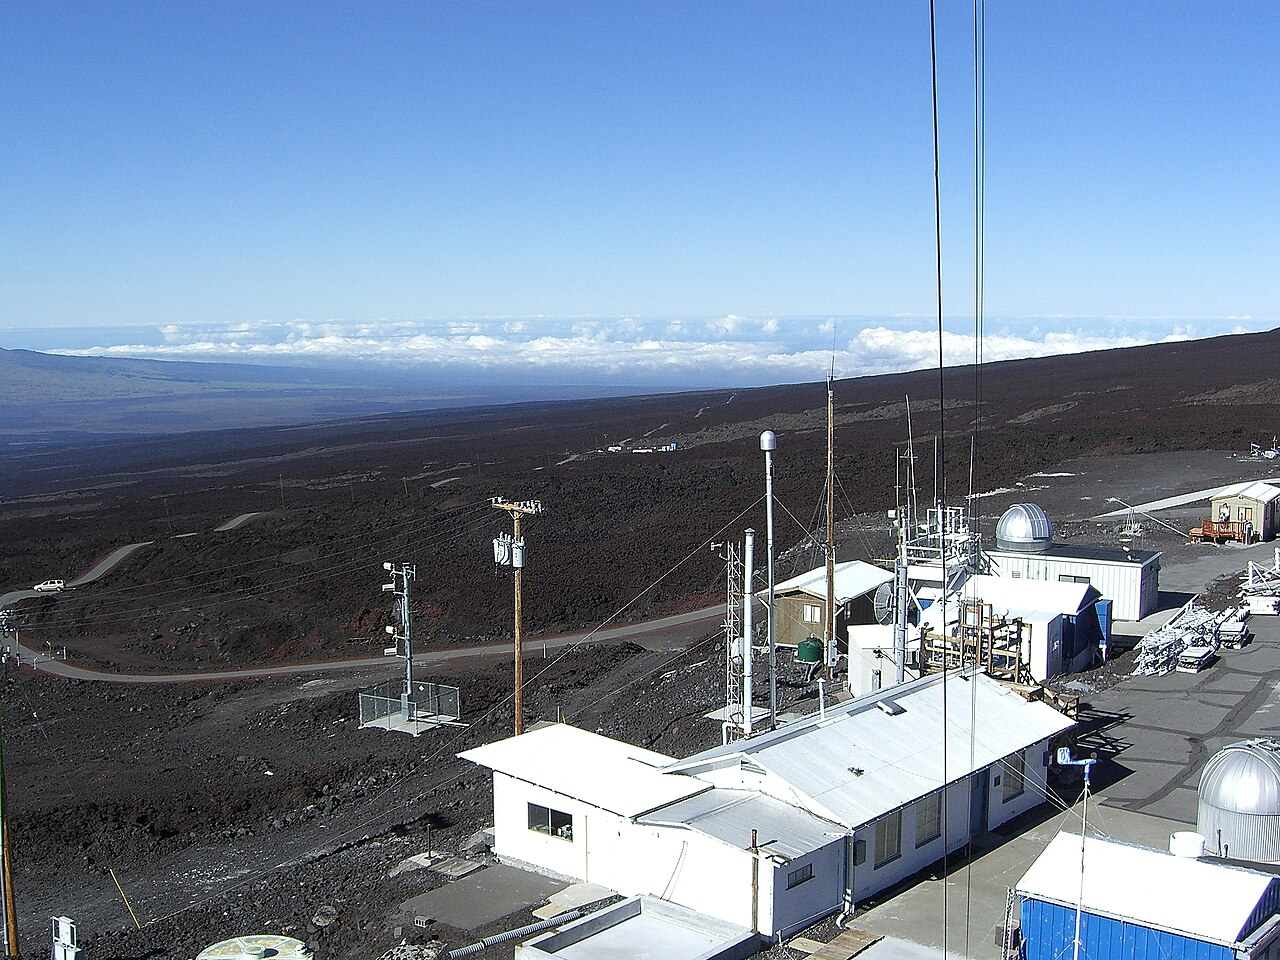
\includegraphics[width=0.56\linewidth]{images/book4/mauna-loa.jpg}\hspace{0.03\linewidth}
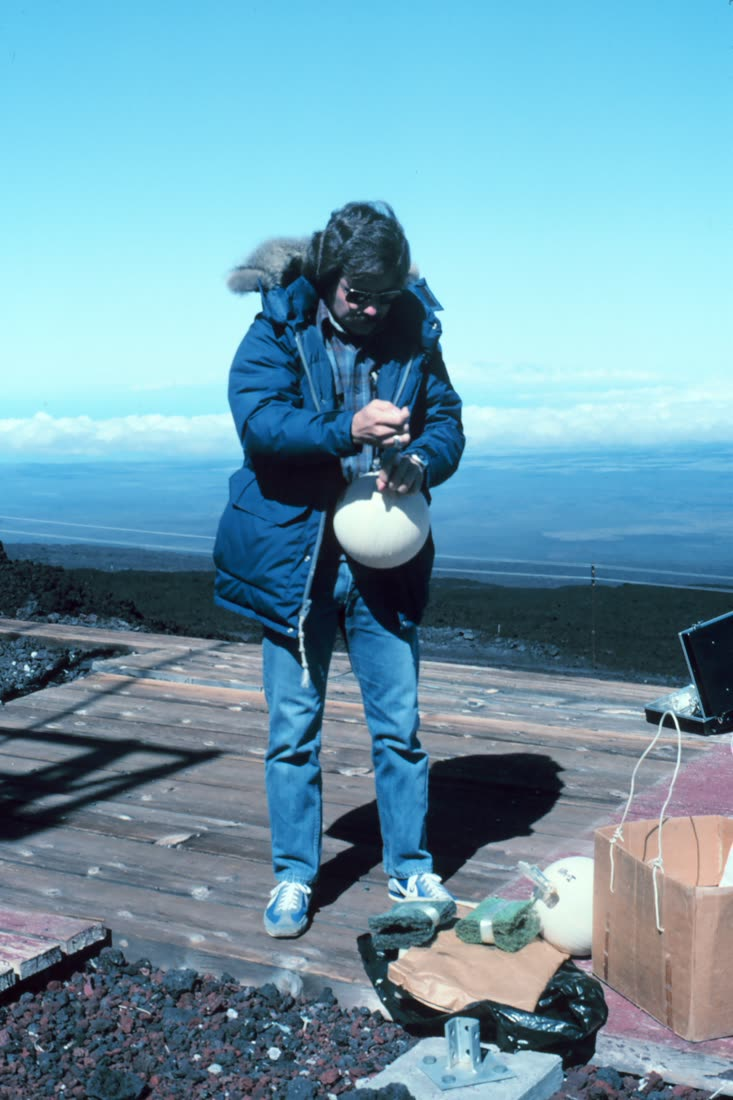
\includegraphics[width=0.33\linewidth]{images/book4/keeling-flask.jpg}

{\small Tempat kurvanya digambar. Kiri: observatorium di lereng utara
Mauna Loa, \qty{3400}{m} di atas, di atas balikan angin pasat yang
menahan udara pulaunya sendiri tetap di bawah. Kanan: sebuah contoh
labu yang diambil pada tahun 1982; labu seperti ini, yang dianalisis di
California, memeriksa penganalisis menerusnya dan diisi di stasiun dari
Alaska sampai Kutub Selatan.}
\end{omfigure}

\section{Daur nitrogennya}

\begin{proposition}[Daur nitrogennya]\label{prop:b2:biogeochemical-cycles:nitrogen}
\index{daur nitrogen}\index{fiksasi nitrogen}\index{nitrifikasi}%
\index{denitrifikasi}\index{proses Haber--Bosch}\index{anamoks}
Nitrogen itu berlimpah --- udaranya menahan $4\times 10^{9}$~Tg
$\mathrm{N_2}$ --- sekaligus langka, karena ikatan rangkap tiga
$\mathrm{N_2}$ hanya dibuka dua proses: petir (beberapa Tg tiap tahun)
dan \emph{\omterm{prop:b2:biogeochemical-cycles:nitrogen}{fiksasi nitrogen} hayati} oleh prokariota bernitrogenase,
sekitar 100 Tg tiap tahun di daratan dan 100 di lautan, dengan ongkos
16 ATP tiap $\mathrm{N_2}$. Nitrogen yang terfiksasi lalu menjalankan
sebuah tangga redoks yang digerakkan mikroba
(\cref{ch:b2:microbial-metabolism}): \emph{amonifikasi} bahan mati
menjadi $\mathrm{NH_4^{+}}$; \emph{nitrifikasi} $\mathrm{NH_4^{+}}$
menjadi $\mathrm{NO_2^{-}}$ dan $\mathrm{NO_3^{-}}$ oleh \omterm{def:b2:microbial-metabolism:trophic}{kemolitotrof}
aerob; penyerapan $\mathrm{NH_4^{+}}$ atau $\mathrm{NO_3^{-}}$ oleh
tumbuhan dan reduksinya kembali menjadi amina; dan, di tempat oksigennya
tidak ada, \emph{\omterm{def:b2:microbial-metabolism:anaerobic}{denitrifikasi}} $\mathrm{NO_3^{-}}$ menjadi
$\mathrm{N_2}$ (dengan $\mathrm{N_2O}$ sebagai sebuah rembesan) serta
\emph{anamoks}, yaitu pengoksidasian amonium secara anaerob oleh nitrit
menjadi $\mathrm{N_2}$, yang bersama-sama mengembalikan kepada udaranya
kira-kira sebanyak yang diambil fiksasinya. \omterm{def:b2:biogeochemical-cycles:reservoir}{Waktu tinggal} sebuah atom
nitrogen di dalam biosfernya adalah beberapa ratus tahun; di dalam
atmosfernya, $4\times
10^{9}/400 \approx 10^{7}$ tahun. Sejak tahun
1913 proses \emph{Haber--Bosch} telah memfiksasi nitrogen secara
industri, kini kira-kira 120 Tg tiap tahun, dan kacang-kacangan yang
dibudidayakan serta pembakaran bahan bakar fosil menambahkan 60 dan 30:
kegiatan manusia memfiksasi nitrogen sebanyak seluruh proses alaminya
bersama-sama, dan memberi makan separuh orang yang hidup.
\end{proposition}

\begin{omfigure}
\begin{tikzpicture}[every node/.style={font=\scriptsize}, >=stealth, box/.style={draw, rounded corners, minimum width=1.9cm, minimum height=0.8cm, align=center, fill=#1}]
  \node[box=omDef!15] (n2) at (0,3.4) {$\mathrm{N_2}$ di udara\\$4\times 10^{9}$ Tg};
  \node[box=omThm!15] (org) at (-4.6,1.0) {N organik\\tumbuhan, tanah, laut};
  \node[box=omProp!15] (nh4) at (-2.2,-0.8) {$\mathrm{NH_4^{+}}$};
  \node[box=omProp!15] (no2) at (2.2,-0.8) {$\mathrm{NO_2^{-}}$};
  \node[box=omProp!15] (no3) at (4.6,1.0) {$\mathrm{NO_3^{-}}$};
  \draw[->, thick] (n2) -- node[above left, align=right] {fiksasi\\nitrogenase, 200\\Haber--Bosch 120} (org);
  \draw[->, thick] (org.south) -- node[below left] {amonifikasi} (nh4.north);
  \draw[->, thick] (nh4) -- node[below] {nitrifikasi} (no2);
  \draw[->, thick] (no2) -- node[below right] {nitrifikasi} (no3);
  \draw[->, thick] (no3) to[bend left=18] node[above, pos=0.72] {asimilasi} (org);
  \draw[->, thick, omExo!80!black] (no3) -- node[above right, align=left] {denitrifikasi\\(anoksik), rembesan $\mathrm{N_2O}$} (n2);
  \draw[->, thick, omExo!80!black] (no2) -- node[right, pos=0.55, align=left] {anamoks\\(dengan $\mathrm{NH_4^{+}}$)} (n2);
  \node[anchor=north, align=center] at (0,-1.5) {fluks dalam Tg N tiap tahun; tiap langkahnya kecuali asimilasi dan amonifikasi dikerjakan prokariota};
\end{tikzpicture}

{\small \omterm{prop:b2:biogeochemical-cycles:nitrogen}{Daur nitrogennya} sebagai sebuah tangga redoks (tumbuhan
mengasimilasi amonium maupun nitrat). Fiksasi dan \omterm{def:b2:microbial-metabolism:anaerobic}{denitrifikasi}, yaitu
kedua pintu menuju atmosfernya, keduanya bersifat mikrob; pintu
industrinya kini menyamai pintu alaminya.}
\end{omfigure}

\begin{proof}[Bukti eksperimental]
Hutan Percobaan Hubbard Brook, New Hampshire: pada tahun 1965 satu
daerah tangkapan air seluruhnya ditebang habis lalu dijaga tetap gundul
dengan herbisida, sementara daerah tetangganya dibiarkan utuh, dan
sungai yang mengalir dari masing-masingnya diukur dan dianalisis selama
bertahun-tahun. Daerah tangkapan yang digunduli kehilangan nitrat pada
enam puluh kali laju kendalinya --- seluruh modal nitrogen tanahnya,
yang tidak lagi diserap tumbuhan, dinitrifikasi lalu tercuci keluar,
membawa kalsium dan kalium bersamanya dan mengasamkan sungainya.
Percobaannya memperlihatkan keketatan daurnya di dalam sebuah hutan
yang utuh (beberapa kilogram nitrogen hilang tiap hektar tiap tahun,
berbanding ratusan yang didaurkan) dan apa yang mematahkannya.
\end{proof}

\section{Fosfor dan belerang}

\begin{proposition}[Dua daur tanpa sebuah gas yang cepat]\label{prop:b2:biogeochemical-cycles:ps}
\index{daur fosfor}\index{daur belerang}\index{eutrofikasi}\index{dimetil sulfida}
\emph{Fosfor} tidak memiliki bentuk gas. Ia masuk ke dalam ekosistemnya
lewat pelapukan apatit di dalam batuan, sekitar 20 Tg tiap tahun di
seluruh permukaan daratannya, didaurkan ulang berkali-kali di dalam
tanah dan danaunya --- sebuah ion fosfat di dalam air permukaan sebuah
danau terserap dalam hitungan jam --- lalu pergi ke endapannya, tempat
ia tinggal selama $10^{8}$ tahun sebuah daur batuan. Karena itu
kehidupan hemat fosfor dan terbatasi fosfor: \omterm{def:b2:biogeochemical-cycles:reservoir}{waktu tinggalnya} di dalam
lautan adalah sekitar \num{20000} tahun, dan fosfat laut dalamnya, yang
dibawa naik pengumbulan air, menetapkan keproduktifannya. Penambangan
kini memindahkan fosfor ke lahan pertanian kira-kira sebanyak yang
dilepaskan pelapukannya, dan limpasannya ke dalam danau menyebabkan
\emph{eutrofikasi}: sebuah ledakan alga, pembusukannya, pemakaian
oksigennya, dan kematian ikannya --- percobaan seluruh danau Schindler
di Ontario pada tahun 1970-an, dengan satu belahan sebuah danau dipupuk
fosfor dan belahan lainnya tidak, memperlihatkan fosfor sajalah yang
menjadi pemicunya, dan membawa kepada penyingkirannya dari deterjen.
\emph{Belerang} memiliki baik sebuah daur batuan (gipsum, pirit) maupun
sebuah fase gas: $\mathrm{SO_2}$ gunung api dan batu bara,
$\mathrm{H_2S}$ endapan anoksik, dan \emph{\omterm{prop:b2:biogeochemical-cycles:ps}{dimetil sulfida}} dari
plankton laut, yang hasil oksidasinya menyemai awan di atas lautannya.
Pembakaran batu bara melipattigakan \omterm{def:b2:biogeochemical-cycles:reservoir}{fluks} belerang ke udaranya pada
abad kedua puluh lalu memberi Eropa dan Amerika Utara hujan asamnya;
penggosok gas membalikkannya dalam beberapa dasawarsa, karena \omterm{def:b2:biogeochemical-cycles:reservoir}{waktu
tinggal} daurnya di udara hanyalah beberapa hari.
\end{proposition}

\begin{omfigure}
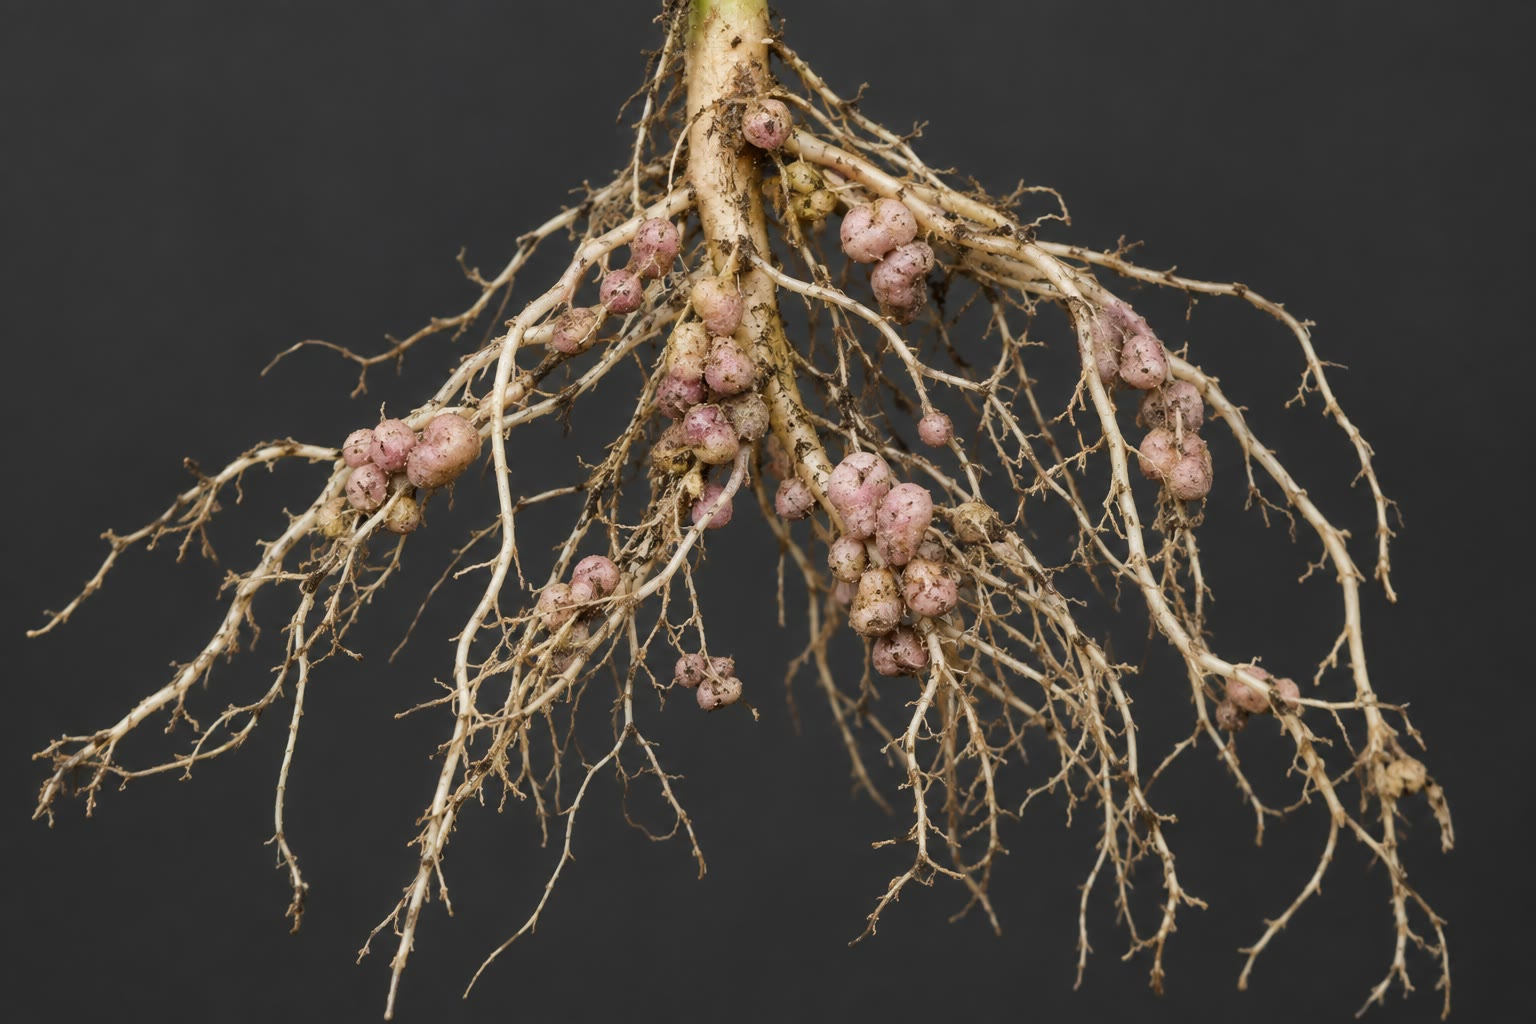
\includegraphics[width=0.44\linewidth]{images/book4/ai/b4-25-root-nodules.jpg}\hspace{0.04\linewidth}
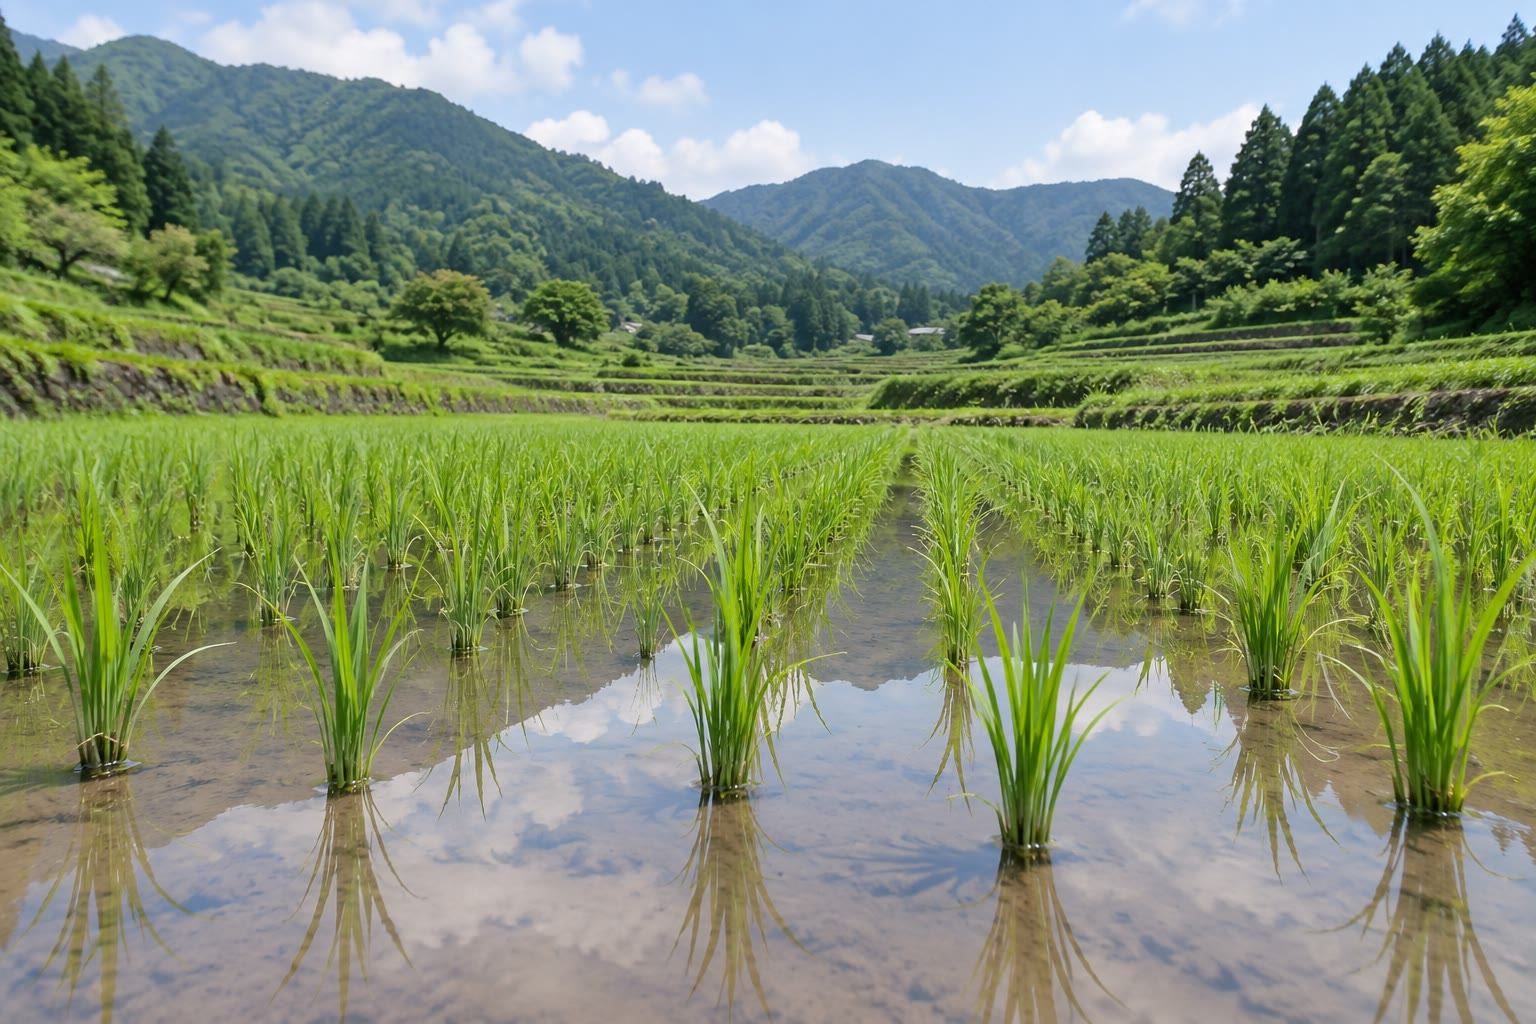
\includegraphics[width=0.44\linewidth]{images/book4/ai/b4-25-rice-paddy.jpg}

{\small Dua pintu \omterm{prop:b2:biogeochemical-cycles:nitrogen}{daur nitrogennya}. Kiri: bintil akar sebuah
kacang-kacangan, yang masing-masingnya adalah sebuah ruang yang di
dalamnya rizobium memfiksasi nitrogen bagi inangnya. Kanan: sebuah
sawah yang tergenang, yang anoksik di bawah permukaannya, yang di
dalamnya \omterm{def:b2:microbial-metabolism:anaerobic}{denitrifikasi} mengembalikan nitrogen ke udaranya dan metanogen
membuat metana.}
\end{omfigure}

\section{Planet yang terusik}

\begin{example}[Apa yang dikatakan angkanya]\label{ex:b2:biogeochemical-cycles:numbers}
Pancaran \qty{10}{GtC} tiap tahun dengan \omterm{prop:b2:biogeochemical-cycles:carbon}{bagian yang mengudara} sebesar
$0.45$ meninggalkan \qty{4.5}{GtC}, atau \qty{2.1}{ppm}, di udaranya
tiap tahun --- yaitu kemiringan yang teramati. Pancaran kumulatif sejak
tahun 1850 adalah kira-kira \qty{700}{GtC}, yang \qty{290}{GtC} darinya
berada di udaranya (140~ppm), dan sisanya di lautan dan daratannya.
Untuk menahan atmosfernya pada aras mana pun, pancaran bersihnya harus
turun sampai sebanyak yang dapat diambil lubuk lambatnya ---
pencampuran laut dalam dan pelapukannya, yang bersama-sama di bawah
\qty{1}{GtC} tiap tahun: \emph{nol bersih} bukanlah sebuah semboyan
melainkan syarat \omterm{def:b2:biogeochemical-cycles:reservoir}{keadaan tunak} \omterm{thm:b2:biogeochemical-cycles:box}{model kotaknya} dengan $\tau$ yang sangat
panjang. Bagi nitrogennya, pelipatduaan \omterm{def:b2:biogeochemical-cycles:reservoir}{fluks} nitrogen yang
terfiksasinya telah melipatduakan nitrat di dalam sungainya,
menghasilkan zona mati di muara Mississippi dan Baltik, dan menaikkan
$\mathrm{N_2O}$ atmosfernya, yaitu sebuah gas rumah kaca dengan \omterm{def:b2:biogeochemical-cycles:reservoir}{waktu
tinggal} seabad, sebesar seperlima. \Cref{ch:b2:global-change} mengikuti
akibatnya bagi makhluk hidup.
\end{example}

\section{Latihan}

\begin{exercise}[$\star$]\label{exo:b2:biogeochemical-cycles:1}
Definisikan \omterm{def:b2:biogeochemical-cycles:reservoir}{tandon}, \omterm{def:b2:biogeochemical-cycles:reservoir}{fluks}, dan \omterm{def:b2:biogeochemical-cycles:reservoir}{waktu tinggal}, lalu hitunglah \omterm{def:b2:biogeochemical-cycles:reservoir}{waktu
tinggal} karbon di dalam tumbuhan darat (450 GtC, dengan fotosintesis
120 GtC tiap tahun) dan di dalam laut dalam (\num{37000} GtC, dengan
pertukaran kira-kira 100 GtC tiap tahun).
\end{exercise}

\begin{exercise}[$\star$]\label{exo:b2:biogeochemical-cycles:2}
Ubahlah \qty{2.5}{ppm} tiap tahun menjadi GtC, dan \qty{10}{GtC}
pancaran menjadi ppm.
\end{exercise}

\begin{exercise}[$\star$]\label{exo:b2:biogeochemical-cycles:3}
Sebutkan kedua proses alami yang membuka $\mathrm{N_2}$, proses yang
mengembalikannya, dan ketiga langkah redoks di antaranya, beserta jasad
yang bertanggung jawab.
\end{exercise}

\begin{exercise}[$\star$]\label{exo:b2:biogeochemical-cycles:4}
Mengapa fosfor lebih sering membatasi keproduktifan daripada nitrogen
sepanjang waktu geologis, sedangkan nitrogen lebih sering daripada
fosfor pada sebuah musim tertentu?
\end{exercise}

\begin{exercise}[$\star\star$]\label{exo:b2:biogeochemical-cycles:5}
Sebuah danau seluas \qty{e7}{m^3} menerima \qty{2}{t} fosfor tiap tahun
dan membilas \qty{20}{\%} airnya tiap tahun. Hitunglah kepekatan fosfor
\omterm{def:b2:biogeochemical-cycles:reservoir}{keadaan tunaknya} dan waktu untuk mencapai \qty{90}{\%} darinya setelah
masukannya bermula. Bagaimana jika masukannya disetengahkan?
\end{exercise}

\begin{exercise}[$\star\star$]\label{exo:b2:biogeochemical-cycles:6}
Dari data Keeling, hitunglah laju pertumbuhan rerata $\mathrm{CO_2}$
pada tahun 1960-an (316 menjadi \qty{325}{ppm} sepanjang sepuluh tahun)
dan pada tahun 2010-an (390 menjadi 411 sepanjang sembilan tahun),
dalam ppm tiap tahun dan dalam GtC tiap tahun.
\end{exercise}

\begin{exercise}[$\star\star$]\label{exo:b2:biogeochemical-cycles:7}
Gigi gergaji musiman di Mauna Loa memiliki amplitudo kira-kira
\qty{6}{ppm} dari puncak ke lembahnya. Ubahlah menjadi GtC lalu
bandingkan dengan produksi primer bersih tahunan daratan belahan bumi
utaranya, yaitu kira-kira \qty{35}{GtC}. Mengapa gigi gergajinya jauh
lebih kecil?
\end{exercise}

\begin{exercise}[$\star\star$]\label{exo:b2:biogeochemical-cycles:8}
Nitrogenase membelanjakan 16 ATP tiap $\mathrm{N_2}$. Bagi sebuah
kacang-kacangan yang memfiksasi \qty{200}{kg} nitrogen tiap hektar tiap
tahun, hitunglah mol $\mathrm{N_2}$ yang terfiksasi dan ATP yang
dibelanjakan, serta massa glukosa yang diwakili ATP itu (kira-kira 30
ATP tiap glukosa). Bagian berapa dari fotosintat sebuah tanaman
\qty{10}{t/ha} itu?
\end{exercise}

\begin{exercise}[$\star\star$]\label{exo:b2:biogeochemical-cycles:9}
Plankton tumbuh pada nisbah Redfield $\mathrm{C:N:P} = 106:16:1$. Air
laut di kedalaman menahan \qty{2.2}{\micro mol/kg} fosfat dan
\qty{32}{\micro mol/kg} nitrat. Mana yang habis lebih dahulu ketika
sebongkah air dibawa ke permukaannya, dan berapa banyak karbon yang
terfiksasi sebelum hal itu terjadi?
\end{exercise}

\begin{exercise}[$\star\star\star$]\label{exo:b2:biogeochemical-cycles:10}
Perlakukan atmosfernya sebagai sebuah kotak dengan karbon berlebih $E$
yang disingkirkan pada laju $E/\tau$ oleh lubuknya dan disuapi pancaran
$Q$. Dengan $\tau =
50$ tahun dan $Q = \qty{10}{GtC/yr}$, berapakah
kelebihan \omterm{def:b2:biogeochemical-cycles:reservoir}{keadaan tunaknya} dan ppm berapa yang bersesuaian dengannya?
Jelaskan mengapa jawaban yang sebenarnya lebih buruk.
\end{exercise}

\begin{exercise}[$\star\star\star$]\label{exo:b2:biogeochemical-cycles:11}
Uji bom melipatduakan $\mathrm{{}^{14}C}$ atmosfernya pada tahun 1963;
kelebihannya lalu turun separuh tiap sekitar 11 tahun, walaupun
$\mathrm{{}^{14}C}$ memiliki paruh waktu 5730 tahun. Jelaskan apa yang
terukur, dan apa yang dikatakan 11 tahun itu kepada Anda tentang \omterm{prop:b2:biogeochemical-cycles:carbon}{daur
karbonnya}.
\end{exercise}

\begin{exercise}[$\star\star\star$]\label{exo:b2:biogeochemical-cycles:12}
``Manusia telah melipatduakan \omterm{prop:b2:biogeochemical-cycles:nitrogen}{daur nitrogennya} dan hanya menyenggol
\omterm{prop:b2:biogeochemical-cycles:carbon}{daur karbonnya}.'' Bahaslah dengan angka: \omterm{def:b2:biogeochemical-cycles:reservoir}{fluks} yang terfiksasi, bagian
dari \omterm{def:b2:biogeochemical-cycles:reservoir}{fluks} alaminya, dan \omterm{def:b2:biogeochemical-cycles:reservoir}{tandon} yang terpengaruh.
\end{exercise}

\section{Soal: Anggaran Karbon Satu Abad}

\begin{problem}[{Soal akhir pekan --- satu abad pancaran dilewatkan
lewat model kotak atmosfernya, bagian lautan dan bagian daratannya,
riam nitrogen dari sebuah ladang yang dipupuk sampai sebuah zona mati,
dan anggaran fosfor sebuah danau, berakhir pada bagian yang mengudara,
kepekatan atmosfer pada tahun 2100, dan nitrogen yang hilang tiap
hektar}]
\label{pb:b2:biogeochemical-cycles:1}
Datanya. Atmosfernya pada tahun 1850: \qty{285}{ppm}; \qty{1}{ppm} $=
\qty{2.13}{GtC}$. Pancaran kumulatif 1850--2020: \qty{700}{GtC};
$\mathrm{CO_2}$ atmosfer pada tahun 2020: \qty{412}{ppm}. Sebuah ladang
seluas \qty{1}{ha} menerima \qty{150}{kg} pupuk nitrogen tiap tahun;
tanamannya menyerap \qty{60}{\%}, \qty{25}{\%} terdenitrifikasi, dan
sisanya tercuci. Sebuah danau seluas \qty{5e7}{m^3} membilas
sepersepuluh airnya tiap tahun dan menerima \qty{5}{t} fosfor tiap tahun.

\medskip
\noindent\textbf{Bagian I --- \omterm{prop:b2:biogeochemical-cycles:carbon}{Bagian yang mengudara}.}
\begin{enumerate}
  \item Hitunglah karbon atmosfernya pada tahun 1850 dan pada tahun
        2020, serta kenaikannya dalam GtC.
  \item Hitunglah \omterm{prop:b2:biogeochemical-cycles:carbon}{bagian yang mengudara} sepanjang 1850--2020.
  \item Di manakah sisanya? Berikan kedua lubuknya dan, dari
        proposisinya, bagian kira-kiranya.
  \item Jika lautannya telah mengambil \qty{25}{\%} pancarannya,
        seberapa besar karbon anorganik terlarutnya, \qty{38000}{GtC},
        telah naik secara nisbi? Mengapa laut permukaannya meskipun
        demikian mengasam secara terukur?
  \item Mengapa \omterm{prop:b2:biogeochemical-cycles:carbon}{bagian yang mengudara} tetap kira-kira tetap sementara
        pancarannya tumbuh secara eksponensial? (Perhatikanlah \omterm{thm:b2:biogeochemical-cycles:box}{model
        kotaknya} dengan $Q \propto e^{t/T}$ dan sebuah lubuk $E/\tau$.)
  \item Akan menjadi berapakah \omterm{prop:b2:biogeochemical-cycles:carbon}{bagian yang mengudara} jika pancarannya
        ditahan tetap selama berabad-abad?
\end{enumerate}

\medskip
\noindent\textbf{Bagian II --- Abad di depannya.}
Modelkan karbon berlebihnya $E$ (di atas aras tahun 1850) dengan
$\mathrm{d}E/\mathrm{d}t = Q - E/\tau$, $\tau = 100$ tahun.
\begin{enumerate}[resume]
  \item Hitunglah kelebihannya pada tahun 2020 dalam GtC.
  \item Dengan $Q$ ditahan pada \qty{10}{GtC/yr}, hitunglah kelebihan
        \omterm{def:b2:biogeochemical-cycles:reservoir}{keadaan tunaknya} dan kepekatan yang disiratkannya.
  \item Selesaikan $E(t)$ dari tahun 2020 dengan $Q = 10$ lalu berikan
        $E$ pada tahun 2100 beserta kepekatannya.
  \item Kini biarkan $Q$ turun secara lurus menjadi nol antara tahun
        2020 dan 2070 lalu tetap nol. Hitunglah $E$ pada tahun 2070
        (integralkan persamaannya; penyelesaian khusus bagi $Q$ yang
        lurus adalah lurus ditambah sebuah tetapan) dan pada tahun 2100.
  \item Bandingkan kedua kepekatannya pada tahun 2100.
  \item Mengapa sebuah $\tau$ tunggal bersifat optimistis bagi skenario
        yang kedua?
\end{enumerate}

\medskip
\noindent\textbf{Bagian III --- Riam nitrogennya.}
\begin{enumerate}[resume]
  \item Hitunglah nitrogen yang diserap tanamannya, yang
        terdenitrifikasi, dan yang tercuci, tiap hektar tiap tahun.
  \item Nitrogen yang tercuci mencapai sebuah sungai sebagai nitrat
        lalu mencapai lautnya, tempat plankton memakainya pada nisbah
        Redfield. Berapa banyak karbon yang ia biarkan difiksasi
        planktonnya?
  \item Karbon itu tenggelam lalu direspirasikan di kedalaman, sehingga
        memakai oksigen sebanyak 1 $\mathrm{O_2}$ tiap C. Hitunglah
        oksigen yang dipakainya, dalam mol dan dalam kilogram.
  \item Satu meter kubik air laut menahan kira-kira \qty{0.25}{mol}
        $\mathrm{O_2}$ ketika jenuh. Berapa meter kubik air dasar yang
        dinyahoksigenkan pencucian satu hektar?
  \item Bagian yang terdenitrifikasi lolos sebagian sebagai
        $\mathrm{N_2O}$, yaitu \qty{1}{\%} nitrogen yang
        terdenitrifikasi. Hitunglah $\mathrm{N_2O}$-nya tiap hektar
        tiap tahun, dan setara pemanasannya dalam $\mathrm{CO_2}$
        ($\mathrm{N_2O}$ adalah 270 kali $\mathrm{CO_2}$ tiap kilogram).
  \item Bandingkan dengan $\mathrm{CO_2}$ yang dipancarkan untuk
        membuat pupuknya (kira-kira \qty{4}{kg} $\mathrm{CO_2}$ tiap
        kilogram nitrogen lewat Haber--Bosch).
\end{enumerate}

\medskip
\noindent\textbf{Bagian IV --- Danaunya.}
\begin{enumerate}[resume]
  \item Hitunglah \omterm{def:b2:biogeochemical-cycles:reservoir}{waktu tinggal} fosfor danaunya jika satu-satunya
        kehilangannya adalah pembilasan, dan kepekatan \omterm{def:b2:biogeochemical-cycles:reservoir}{keadaan
        tunaknya} dalam \unit{mg/m^3}.
  \item Danau dengan fosfor lebih dari \qty{30}{mg/m^3} bersifat
        eutrof. Apakah danau ini demikian?
  \item Pengendapan menyingkirkan fosfor dengan tetapan waktunya
        sendiri sebesar 5 tahun. Hitung ulang \omterm{def:b2:biogeochemical-cycles:reservoir}{waktu tinggalnya} dan
        kepekatannya.
  \item Masukannya dipangkas menjadi \qty{1}{t} tiap tahun. Hitunglah
        \omterm{def:b2:biogeochemical-cycles:reservoir}{keadaan tunaknya} yang baru dan waktu untuk mencapai dalam
        \qty{10}{\%} darinya.
  \item Mengapa banyak danau pulih lebih lambat daripada yang
        diramalkan perhitungan ini?
  \item Hitunglah karbon yang dapat dibangun fosfor danaunya menjadi
        plankton tiap tahun pada nisbah Redfield, dari masukan
        \qty{5}{t}-nya.
  \item Nyatakan hasilnya: \omterm{prop:b2:biogeochemical-cycles:carbon}{bagian yang mengudara}, kedua kepekatannya
        pada tahun 2100, dan nitrogen yang tercuci tiap hektar.
\end{enumerate}
\end{problem}
